\documentclass[10pt]{article}
\usepackage[polish]{babel}
\usepackage[utf8]{inputenc}
\usepackage[T1]{fontenc}
\usepackage{graphicx}
\usepackage[export]{adjustbox}
\graphicspath{ {./images/} }
\usepackage{amsmath}
\usepackage{amsfonts}
\usepackage{amssymb}
\usepackage[version=4]{mhchem}
\usepackage{stmaryrd}

\title{PRÓBNY EGZAMIN MATURALNY \\
 Z MATEMATYKI }

\author{}
\date{}


\begin{document}
\maketitle
\begin{center}

\includegraphics[max width=\textwidth]{2024_11_21_ad52a81220b9b2239458g-01(3)}
\end{center}

\begin{center}
\begin{tabular}{|c|}
\hline
\begin{tabular}{c}
Miejsce \\
na naklejke \\
\end{tabular} \\
\hline
\end{tabular}
\end{center}

\section*{LISTOPAD ROK 2009}
\section*{POZIOM PODSTAWOWY}
\section*{Czas pracy 170 minut}
\section*{Instrukcja dla zdającego}
\begin{enumerate}
  \item Sprawdź, czy arkusz egzaminacyjny zawiera 17 stron (zadania 1-34). Ewentualny brak zgłoś przewodniczącemu zespołu nadzorującego egzamin.
  \item Rozwiązania zadań i odpowiedzi zamieść w miejscu na to przeznaczonym.
  \item Odpowiedzi do zadań zamkniętych przenieś na kartę odpowiedzi, zaznaczając je w części karty przeznaczonej dla zdającego. Zamaluj \(\square\) pola do tego przeznaczone. Błędne zaznaczenie otocz kółkiem i zaznacz właściwe.
  \item Pamiętaj, że pominięcie argumentacji lub istotnych obliczeń w rozwiązaniu zadania otwartego może spowodować, że za to rozwiązanie możesz nie dostać pełnej liczby punktów.
  \item Pisz czytelnie. Używaj długopisu lub pióra tylko z czarnym tuszem lub atramentem.
  \item Nie używaj korektora, a błędne zapisy przekreśl.
  \item Pamiętaj, że zapisy w brudnopisie nie podlegają ocenie.
  \item Możesz korzystać z zestawu wzorów matematycznych, cyrkla i linijki oraz kalkulatora.
  \item Na karcie odpowiedzi wpisz swoją datę urodzenia i PESEL. Nie wpisuj żadnych znaków w części przeznaczonej dla egzaminatora.\\

\includegraphics[max width=\textwidth, center]{2024_11_21_ad52a81220b9b2239458g-01(2)}
\end{enumerate}

Za rozwiązanie wszystkich zadań można otrzymać łacznie 50 punktów

Życzymy powodzenia!

Wypelnia zdający przed rozpoczęciem pracy\\
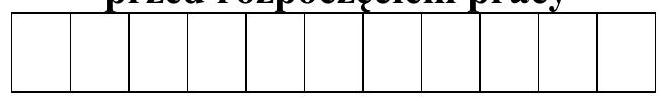
\includegraphics[max width=\textwidth, center]{2024_11_21_ad52a81220b9b2239458g-01}

PESEL ZDAJĄCEGO\\

\includegraphics[max width=\textwidth, center]{2024_11_21_ad52a81220b9b2239458g-01(1)}

\section*{ZADANIA ZAMKNIĘTE}
\section*{W zadaniach od 1. do 25. wybierz i zaznacz na karcie odpowiedzi jedna}
poprawnq odpowiedź.

\section*{Zadanie 1. (1 pkt)}
Wskaż nierówność, która opisuje sumę przedziałów zaznaczonych na osi liczbowej.\\
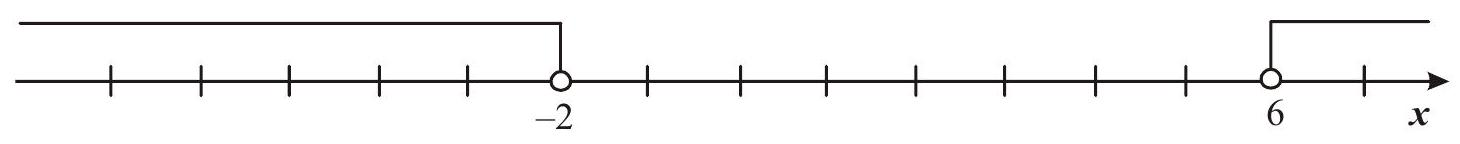
\includegraphics[max width=\textwidth, center]{2024_11_21_ad52a81220b9b2239458g-02}\\
A. \(|x-2|>4\)\\
B. \(|x-2|<4\)\\
C. \(|x-4|<2\)\\
D. \(|x-4|>2\)

\section*{Zadanie 2. (1 pkt)}
Na seans filmowy sprzedano 280 biletów, w tym 126 ulgowych. Jaki procent sprzedanych biletów stanowiły bilety ulgowe?\\
A. \(22 \%\)\\
B. \(33 \%\)\\
C. \(45 \%\)\\
D. \(63 \%\)

\section*{Zadanie 3. (1 pkt)}
\(6 \%\) liczby \(x\) jest równe 9 . Wtedy\\
A. \(x=240\)\\
B. \(x=150\)\\
C. \(x=24\)\\
D. \(x=15\)

Zadanie 4. (1 pkt)\\
Iloraz \(32^{-3}:\left(\frac{1}{8}\right)^{4}\) jest równy\\
A. \(2^{-27}\)\\
B. \(2^{-3}\)\\
C. \(2^{3}\)\\
D. \(2^{27}\)

\section*{Zadanie 5. (1 pkt)}
O liczbie \(x\) wiadomo, że \(\log _{3} x=9\). Zatem\\
A. \(x=2\)\\
B. \(x=\frac{1}{2}\)\\
C. \(x=3^{9}\)\\
D. \(x=9^{3}\)

\section*{Zadanie 6. (1 pkt)}
Wyrażenie \(27 x^{3}+y^{3}\) jest równe iloczynowi\\
A. \((3 x+y)\left(9 x^{2}-3 x y+y^{2}\right)\)\\
B. \((3 x+y)\left(9 x^{2}+3 x y+y^{2}\right)\)\\
C. \((3 x-y)\left(9 x^{2}+3 x y+y^{2}\right)\)\\
D. \((3 x-y)\left(9 x^{2}-3 x y+y^{2}\right)\)

\section*{Zadanie 7. (1 pkt)}
Dane są wielomiany: \(W(x)=x^{3}-3 x+1\) oraz \(V(x)=2 x^{3}\). Wielomian \(W(x) \cdot V(x)\) jest równy\\
A. \(2 x^{5}-6 x^{4}+2 x^{3}\)\\
B. \(2 x^{6}-6 x^{4}+2 x^{3}\)\\
C. \(2 x^{5}+3 x+1\)\\
D. \(2 x^{5}+6 x^{4}+2 x^{3}\)

\section*{BRUDNOPIS}
\section*{Zadanie \(8 . \quad(1\) pkt)}
Wierzchołek paraboli o równaniu \(y=-3(x+1)^{2}\) ma współrzędne\\
A. \((-1,0)\)\\
B. \((0,-1)\)\\
C. \((1,0)\)\\
D. \((0,1)\)

\section*{Zadanie 9. (1 pkt)}
Do wykresu funkcji \(f(x)=x^{2}+x-2\) należy punkt\\
A. \((-1,-4)\)\\
B. \((-1,1)\)\\
C. \((-1,-1)\)\\
D. \((-1,-2)\)

Zadanie 10. (1 pkt)\\
Rozwiązaniem równania \(\frac{x-5}{x+3}=\frac{2}{3}\) jest liczba\\
A. 21\\
B. 7\\
C. \(\frac{17}{3}\)\\
D. 0

\section*{Zadanie 11. (1 pkt)}
Zbiór rozwiązań nierówności \((x+1)(x-3)>0\) przedstawiony jest na rysunku\\
A.\\
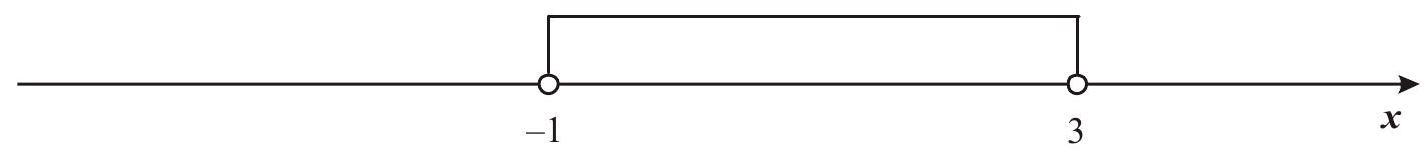
\includegraphics[max width=\textwidth, center]{2024_11_21_ad52a81220b9b2239458g-04(1)}\\
B.\\
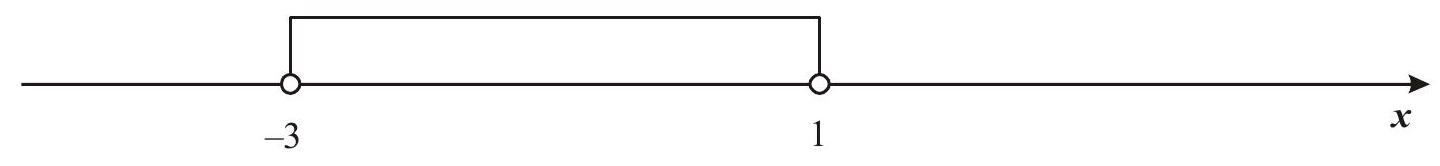
\includegraphics[max width=\textwidth, center]{2024_11_21_ad52a81220b9b2239458g-04(2)}\\
C.\\
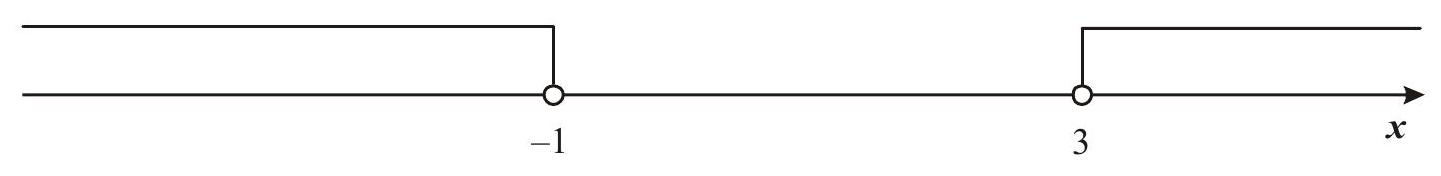
\includegraphics[max width=\textwidth, center]{2024_11_21_ad52a81220b9b2239458g-04}\\
D.\\
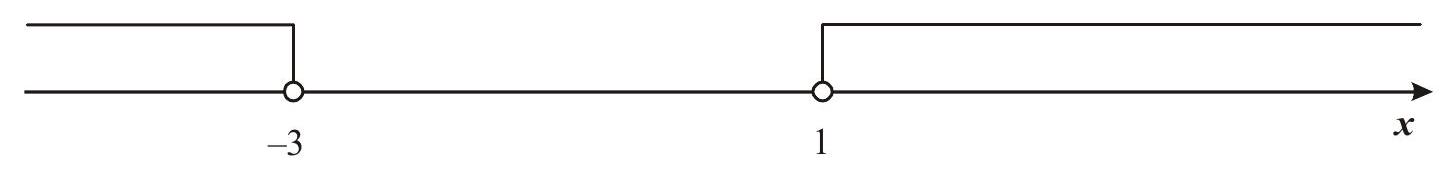
\includegraphics[max width=\textwidth, center]{2024_11_21_ad52a81220b9b2239458g-04(3)}

Zadanie 12. (1 pkt)\\
Dla \(n=1,2,3, \ldots\) ciag \(\left(a_{n}\right)\) jest określony wzorem: \(a_{n}=(-1)^{n} \cdot(3-n)\). Wtedy\\
A. \(a_{3}<0\)\\
B. \(a_{3}=0\)\\
C. \(a_{3}=1\)\\
D. \(a_{3}>1\)

\section*{Zadanie 13. (1 pkt)}
W ciągu arytmetycznym trzeci wyraz jest równy 14, a jedenasty jest równy 34. Różnica tego ciagu jest równa\\
A. 9\\
B. \(\frac{5}{2}\)\\
C. 2\\
D. \(\frac{2}{5}\)

\section*{Zadanie 14. (1 pkt)}
W ciagu geometrycznym \(\left(a_{n}\right)\) dane sa: \(a_{1}=32\) i \(a_{4}=-4\). Iloraz tego ciagu jest równy\\
A. 12\\
B. \(\frac{1}{2}\)\\
C. \(-\frac{1}{2}\)\\
D. -12

\section*{BRUDNOPIS}
\section*{Zadanie 15. (1 pkt)}
Kąt \(\alpha\) jest ostry i \(\sin \alpha=\frac{8}{9}\). Wtedy \(\cos \alpha\) jest równy\\
A. \(\frac{1}{9}\)\\
B. \(\frac{8}{9}\)\\
C. \(\frac{\sqrt{17}}{9}\)\\
D. \(\frac{\sqrt{65}}{9}\)

Zadanie 16. (1 pkt)\\
Dany jest trójkąt prostokątny (patrz rysunek). Wtedy \(\operatorname{tg} \alpha\) jest równy\\
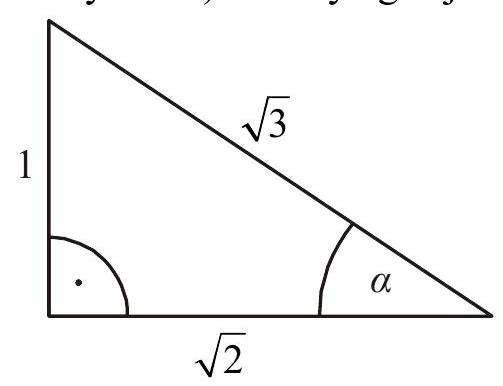
\includegraphics[max width=\textwidth, center]{2024_11_21_ad52a81220b9b2239458g-06}\\
A. \(\sqrt{2}\)\\
B. \(\frac{\sqrt{2}}{\sqrt{3}}\)\\
C. \(\frac{\sqrt{3}}{\sqrt{2}}\)\\
D. \(\frac{1}{\sqrt{2}}\)

\section*{Zadanie 17. (1 pkt)}
W trójkącie równoramiennym \(A B C\) dane są \(|A C|=|B C|=7\) oraz \(|A B|=12\). Wysokość opuszczona z wierzchołka \(C\) jest równa\\
A. \(\sqrt{13}\)\\
B. \(\sqrt{5}\)\\
C. 1\\
D. 5

Zadanie 18. (1 pkt)\\
Oblicz długość odcinka \(A E\) wiedząc, że \(A B \| C D\) i \(|A B|=6,|A C|=4,|C D|=8\).\\
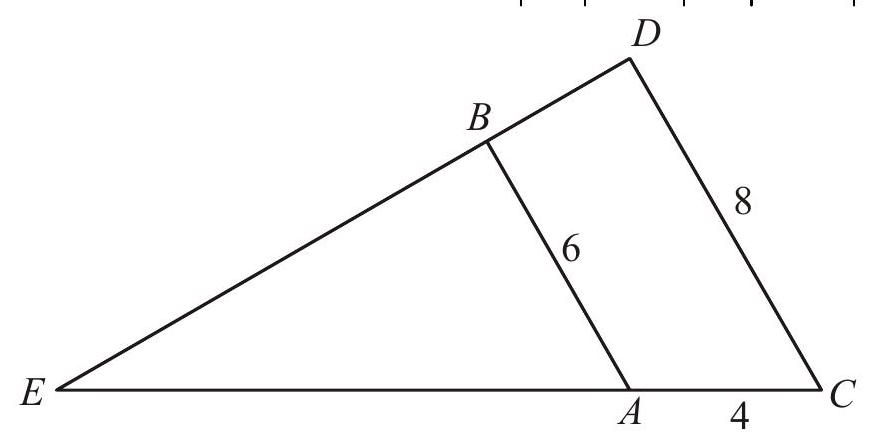
\includegraphics[max width=\textwidth, center]{2024_11_21_ad52a81220b9b2239458g-06(1)}\\
A. \(|A E|=2\)\\
B. \(|A E|=4\)\\
C. \(|A E|=6\)\\
D. \(|A E|=12\)

Zadanie 19. (1 pkt)\\
Dane są punkty \(A=(-2,3)\) oraz \(B=(4,6)\). Długość odcinka \(A B\) jest równa\\
A. \(\sqrt{208}\)\\
B. \(\sqrt{52}\)\\
C. \(\sqrt{45}\)\\
D. \(\sqrt{40}\)

Zadanie 20. (1 pkt)\\
Promień okręgu o równaniu \((x-1)^{2}+y^{2}=16\) jest równy\\
A. 1\\
B. 2\\
C. 3\\
D. 4

\section*{BRUDNOPIS}
\section*{Zadanie 21. (1 pkt)}
Wykres funkcji liniowej określonej wzorem \(f(x)=3 x+2\) jest prostą prostopadłą do prostej o równaniu:\\
A. \(y=-\frac{1}{3} x-1\)\\
B. \(y=\frac{1}{3} x+1\)\\
C. \(y=3 x+1\)\\
D. \(y=3 x-1\)

\section*{Zadanie 22. (1 pkt)}
Prosta o równaniu \(y=-4 x+(2 m-7)\) przechodzi przez punkt \(A=(2,-1)\). Wtedy\\
A. \(m=7\)\\
B. \(m=2 \frac{1}{2}\)\\
C. \(m=-\frac{1}{2}\)\\
D. \(m=-17\)

Zadanie 23. (1 pkt)\\
Pole powierzchni całkowitej sześcianu jest równe \(150 \mathrm{~cm}^{2}\). Długość krawędzi tego sześcianu jest równa\\
A. \(3,5 \mathrm{~cm}\)\\
B. 4 cm\\
C. \(4,5 \mathrm{~cm}\)\\
D. 5 cm

Zadanie 24. (1 pkt)\\
Średnia arytmetyczna pięciu liczb: \(5, x, 1,3,1\) jest równa 3 . Wtedy\\
A. \(x=2\)\\
B. \(x=3\)\\
C. \(x=4\)\\
D. \(x=5\)

\section*{Zadanie 25. (1 pkt)}
Wybieramy liczbę \(a\) ze zbioru \(A=\{2,3,4,5\}\) oraz liczbę \(b\) ze zbioru \(B=\{1,4\}\). Ile jest takich par \((a, b)\), że iloczyn \(a \cdot b\) jest liczbą nieparzystą?\\
A. 2\\
B. 3\\
C. 5\\
D. 20

\section*{BRUDNOPIS}
\begin{center}

\includegraphics[max width=\textwidth]{2024_11_21_ad52a81220b9b2239458g-09}
\end{center}

\section*{ZADANIA OTWARTE}
\section*{Rozwiazania zadań o numerach od 26. do 34. należ̀y zapisać w wyznaczonych miejscach pod treścia zadania.}
Zadanie 26. (2 pkt)\\
Rozwiąż nierówność \(x^{2}-3 x+2 \leq 0\).\\

\includegraphics[max width=\textwidth, center]{2024_11_21_ad52a81220b9b2239458g-10}

Odpowiedź:\\
Zadanie 27. (2 pkt)\\
Rozwiąż równanie \(x^{3}-7 x^{2}+2 x-14=0\).

\begin{center}
\begin{tabular}{|c|c|c|c|c|c|c|c|c|c|c|c|c|c|c|c|c|c|c|c|c|c|c|c|c|c|c|c|c|c|c|}
\hline
 &  &  &  &  &  &  &  &  &  &  &  &  &  &  &  &  &  &  &  &  &  &  &  &  &  &  &  &  &  &  \\
\hline
 &  &  &  &  &  &  &  &  &  &  &  &  &  &  &  &  &  &  &  &  &  &  &  &  &  &  &  &  &  &  \\
\hline
 &  &  &  &  &  &  &  &  &  &  &  &  &  &  &  &  &  &  &  &  &  &  &  &  &  &  &  &  &  &  \\
\hline
 &  &  &  &  &  &  &  &  &  &  &  &  &  &  &  &  &  &  &  &  &  &  &  &  &  &  &  &  &  &  \\
\hline
 &  &  &  &  &  &  &  &  &  &  &  &  &  &  &  &  &  &  &  &  &  &  &  &  &  &  &  &  &  &  \\
\hline
 &  &  &  &  &  &  &  &  &  &  &  &  &  &  &  &  &  &  &  &  &  &  &  &  &  &  &  &  &  &  \\
\hline
 &  &  &  &  &  &  &  &  &  &  &  &  &  &  &  &  &  &  &  &  &  &  &  &  &  &  &  &  &  &  \\
\hline
 &  &  &  &  &  &  &  &  &  &  &  &  &  &  &  &  &  &  &  &  &  &  &  &  &  &  &  &  &  &  \\
\hline
 &  &  &  &  &  &  &  &  &  &  &  &  &  &  &  &  &  &  &  &  &  &  &  &  &  &  &  &  &  &  \\
\hline
 &  &  &  &  &  &  &  &  &  &  &  &  &  &  &  &  &  &  &  &  &  &  &  &  &  &  &  &  &  &  \\
\hline
 &  &  &  &  &  &  &  &  &  &  &  &  &  &  &  &  &  &  &  &  &  &  &  &  &  &  &  &  &  &  \\
\hline
 &  &  &  &  &  &  &  &  &  &  &  &  &  &  &  &  &  &  &  &  &  &  &  &  &  &  &  &  &  &  \\
\hline
 &  &  &  &  &  &  &  &  &  &  &  &  &  &  &  &  &  &  &  &  &  &  &  &  &  &  &  &  &  &  \\
\hline
 &  &  &  &  &  &  &  &  &  &  &  &  &  &  &  &  &  &  &  &  &  &  &  &  &  &  &  &  &  &  \\
\hline
 &  &  &  &  &  &  &  &  &  &  &  &  &  &  &  &  &  &  &  &  &  &  &  &  &  &  &  &  &  &  \\
\hline
 &  &  &  &  &  &  &  &  &  &  &  &  &  &  &  &  &  &  &  &  &  &  &  &  &  &  &  &  &  &  \\
\hline
 &  &  &  &  &  &  &  &  &  &  &  &  &  &  &  &  &  &  &  &  &  &  &  &  &  &  &  &  &  &  \\
\hline
 &  &  &  &  &  &  &  &  &  &  &  &  &  &  &  &  &  &  &  &  &  &  &  &  &  &  &  &  &  &  \\
\hline
 &  &  &  &  &  &  &  &  &  &  &  &  &  &  &  &  &  &  &  &  &  &  &  &  &  &  &  &  &  &  \\
\hline
\end{tabular}
\end{center}

Odpowiedź:

Zadanie 28. (2 pkt)\\
W układzie współrzędnych na płaszczyźnie punkty \(A=(2,5)\) i \(\mathrm{C}=(6,7)\) są przeciwległymi wierzchołkami kwadratu \(A B C D\). Wyznacz równanie prostej \(B D\).\\

\includegraphics[max width=\textwidth, center]{2024_11_21_ad52a81220b9b2239458g-11(1)}

Odpowiedź:

Zadanie 29. (2 pkt)\\
Kat \(\alpha\) jest ostry i \(\operatorname{tg} \alpha=\frac{4}{3}\). Oblicz \(\sin \alpha+\cos \alpha\).\\

\includegraphics[max width=\textwidth, center]{2024_11_21_ad52a81220b9b2239458g-11}

Odpowiedź:

Zadanie 30. (2 pkt)\\
Wykaż, że dla każdego \(m\) ciag \(\left(\frac{m+1}{4}, \frac{m+3}{6}, \frac{m+9}{12}\right)\) jest arytmetyczny.

\begin{center}
\begin{tabular}{|c|c|c|c|c|c|c|c|c|c|c|c|c|c|c|c|c|c|c|c|c|c|c|}
\hline
 &  &  &  &  &  &  &  &  &  &  &  &  &  &  &  &  &  &  &  &  &  &  \\
\hline
 &  &  &  &  &  &  &  &  &  &  &  &  &  &  &  &  &  &  &  &  &  &  \\
\hline
 &  &  &  &  &  &  &  &  &  &  &  &  &  &  &  &  &  &  &  &  &  &  \\
\hline
 &  &  &  &  &  &  &  &  &  &  &  &  &  &  &  &  &  &  &  &  &  &  \\
\hline
 &  &  &  &  &  &  &  &  &  &  &  &  &  &  &  &  &  &  &  &  &  &  \\
\hline
 &  &  &  &  &  &  &  &  &  &  &  &  &  &  &  &  &  &  &  &  &  &  \\
\hline
 &  &  &  &  &  &  &  &  &  &  &  &  &  &  &  &  &  &  &  &  &  &  \\
\hline
 &  &  &  &  &  &  &  &  &  &  &  &  &  &  &  &  &  &  &  &  &  &  \\
\hline
 &  &  &  &  &  &  &  &  &  &  &  &  &  &  &  &  &  &  &  &  &  &  \\
\hline
 &  &  &  &  &  &  &  &  &  &  &  &  &  &  &  &  &  &  &  &  &  &  \\
\hline
 &  &  &  &  &  &  &  &  &  &  &  &  &  &  &  &  &  &  &  &  &  &  \\
\hline
 &  &  &  &  &  &  &  &  &  &  &  &  &  &  &  &  &  &  &  &  &  &  \\
\hline
 &  &  &  &  &  &  &  &  &  &  &  &  &  &  &  &  &  &  &  &  &  &  \\
\hline
 &  &  &  &  &  &  &  &  &  &  &  &  &  &  &  &  &  &  &  &  &  &  \\
\hline
 &  &  &  &  &  &  &  &  &  &  &  &  &  &  &  &  &  &  &  &  &  &  \\
\hline
 &  &  &  &  &  &  &  &  &  &  &  &  &  &  &  &  &  &  &  &  &  &  \\
\hline
 &  &  &  &  &  &  &  &  &  &  &  &  &  &  &  &  &  &  &  &  &  &  \\
\hline
 &  &  &  &  &  &  &  &  &  &  &  &  &  &  &  &  &  &  &  &  &  &  \\
\hline
 &  &  &  &  &  &  &  &  &  &  &  &  &  &  &  &  &  &  &  &  &  &  \\
\hline
 &  &  &  &  &  &  &  &  &  &  &  &  &  &  &  &  &  &  &  &  &  &  \\
\hline
 &  &  &  &  &  &  &  &  &  &  &  &  &  &  &  &  &  &  &  &  &  &  \\
\hline
 &  &  &  &  &  &  &  &  &  &  &  &  &  &  &  &  &  &  &  &  &  &  \\
\hline
 &  &  &  &  &  &  &  &  &  &  &  &  &  &  &  &  &  &  &  &  &  &  \\
\hline
 &  &  &  &  &  &  &  &  &  &  &  &  &  &  &  &  &  &  &  &  &  &  \\
\hline
 &  &  &  &  &  &  &  &  &  &  &  &  &  &  &  &  &  &  &  &  &  &  \\
\hline
 &  &  &  &  &  &  &  &  &  &  &  &  &  &  &  &  &  &  &  &  &  &  \\
\hline
 &  &  &  &  &  &  &  &  &  &  &  &  &  &  &  &  &  &  &  &  &  &  \\
\hline
 &  &  &  &  &  &  &  &  &  &  &  &  &  &  &  &  &  &  &  &  &  &  \\
\hline
 &  &  &  &  &  &  &  &  &  &  &  &  &  &  &  &  &  &  &  &  &  &  \\
\hline
 &  &  &  &  &  &  &  &  &  &  &  &  &  &  &  &  &  &  &  &  &  &  \\
\hline
 &  &  &  &  &  &  &  &  &  &  &  &  &  &  &  &  &  &  &  &  &  &  \\
\hline
 &  &  &  &  &  &  &  &  &  &  &  &  &  &  &  &  &  &  &  &  &  &  \\
\hline
 &  &  &  &  &  &  &  &  &  &  &  &  &  &  &  &  &  &  &  &  &  &  \\
\hline
 &  &  &  &  &  &  &  &  &  &  &  &  &  &  &  &  &  &  &  &  &  &  \\
\hline
 &  &  &  &  &  &  &  &  &  &  &  &  &  &  &  &  &  &  &  &  &  &  \\
\hline
 &  &  &  &  &  &  &  &  &  &  &  &  &  &  &  &  &  &  &  &  &  &  \\
\hline
 &  &  &  &  &  &  &  &  &  &  &  &  &  &  &  &  &  &  &  &  &  &  \\
\hline
 &  &  &  &  &  &  &  &  &  &  &  &  &  &  &  &  &  &  &  &  &  &  \\
\hline
 &  &  &  &  &  &  &  &  &  &  &  &  &  &  &  &  &  &  &  &  &  &  \\
\hline
 &  &  &  &  &  &  &  &  &  &  &  &  &  &  &  &  &  &  &  &  &  &  \\
\hline
 &  &  &  &  &  &  &  &  &  &  &  &  &  &  &  &  &  &  &  &  &  &  \\
\hline
 &  &  &  &  &  &  &  &  &  &  &  &  &  &  &  &  &  &  &  &  &  &  \\
\hline
 &  &  &  &  &  &  &  &  &  &  &  &  &  &  &  &  &  &  &  &  &  &  \\
\hline
 &  &  &  &  &  &  &  &  &  &  &  &  &  &  &  &  &  &  &  &  &  &  \\
\hline
 &  &  &  &  &  &  &  &  &  &  &  &  &  &  &  &  &  &  &  &  &  &  \\
\hline
\end{tabular}
\end{center}

Zadanie 31. (2 pkt)\\
Trójkąty \(A B C\) i \(C D E\) są równoboczne. Punkty \(A, C\) i \(E\) leżą na jednej prostej. Punkty \(K, L\) i \(M\) są środkami odcinków \(A C, C E\) i \(B D\) (zobacz rysunek). Wykaż, że punkty \(K, L\) i \(M\) są wierzchołkami trójkąta równobocznego.\\
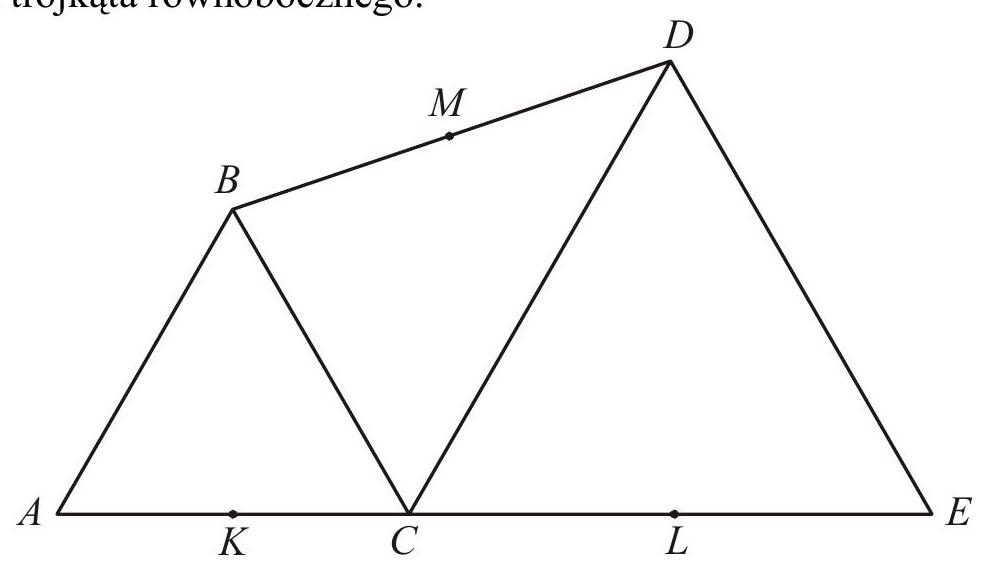
\includegraphics[max width=\textwidth, center]{2024_11_21_ad52a81220b9b2239458g-13}\\

\includegraphics[max width=\textwidth, center]{2024_11_21_ad52a81220b9b2239458g-13(1)}

\section*{Zadanie 32. (5 pkt)}
Uczeń przeczytał książkę liczącą 480 stron, przy czym każdego dnia czytał jednakową liczbę stron. Gdyby czytał każdego dnia o 8 stron więcej, to przeczytałby tę książkę o 3 dni wcześniej. Oblicz, ile dni uczeń czytał tę książkę.\\

\includegraphics[max width=\textwidth, center]{2024_11_21_ad52a81220b9b2239458g-14}

Odpowiedź:

Zadanie 33. (4 pkt)\\
Punkty \(A=(2,0)\) i \(B=(12,0)\) są wierzchołkami trójkąta prostokątnego \(A B C\) o przeciwprostokątnej \(A B\). Wierzchołek \(C\) leży na prostej o równaniu \(y=x\). Oblicz współrzędne punktu \(C\).

\begin{center}
\begin{tabular}{|c|c|c|c|c|c|c|c|c|c|c|c|c|c|c|c|c|c|c|c|c|c|c|}
\hline
 &  &  &  &  &  &  &  &  &  &  &  &  &  &  &  &  &  &  &  &  &  &  \\
\hline
 &  &  &  &  &  &  &  &  &  &  &  &  &  &  &  &  &  &  &  &  &  &  \\
\hline
 &  &  &  &  &  &  &  &  &  &  &  &  &  &  &  &  &  &  &  &  &  &  \\
\hline
 &  &  &  &  &  &  &  &  &  &  &  &  &  &  &  &  &  &  &  &  &  &  \\
\hline
 &  &  &  &  &  &  &  &  &  &  &  &  &  &  &  &  &  &  &  &  &  &  \\
\hline
 &  &  &  &  &  &  &  &  &  &  &  &  &  &  &  &  &  &  &  &  &  &  \\
\hline
 &  &  &  &  &  &  &  &  &  &  &  &  &  &  &  &  &  &  &  &  &  &  \\
\hline
 &  &  &  &  &  &  &  &  &  &  &  &  &  &  &  &  &  &  &  &  &  &  \\
\hline
 &  &  &  &  &  &  &  &  &  &  &  &  &  &  &  &  &  &  &  &  &  &  \\
\hline
 &  &  &  &  &  &  &  &  &  &  &  &  &  &  &  &  &  &  &  &  &  &  \\
\hline
 &  &  &  &  &  &  &  &  &  &  &  &  &  &  &  &  &  &  &  &  &  &  \\
\hline
 &  &  &  &  &  &  &  &  &  &  &  &  &  &  &  &  &  &  &  &  &  &  \\
\hline
 &  &  &  &  &  &  &  &  &  &  &  &  &  &  &  &  &  &  &  &  &  &  \\
\hline
 &  &  &  &  &  &  &  &  &  &  &  &  &  &  &  &  &  &  &  &  &  &  \\
\hline
- &  &  &  &  &  &  &  &  &  &  &  &  &  &  &  &  &  &  &  &  &  &  \\
\hline
 &  &  &  &  &  &  &  &  &  &  &  &  &  &  &  &  &  &  &  &  &  &  \\
\hline
 &  &  &  &  &  &  &  &  &  &  &  &  &  &  &  &  &  &  &  &  &  &  \\
\hline
 &  &  &  &  &  &  &  &  &  &  &  &  &  &  &  &  &  &  &  &  &  &  \\
\hline
 &  &  &  &  &  &  &  &  &  &  &  &  &  &  &  &  &  &  &  &  &  &  \\
\hline
 &  &  &  &  &  &  &  &  &  &  &  &  &  &  &  &  &  &  &  &  &  &  \\
\hline
 &  &  &  &  &  &  &  &  &  &  &  &  &  &  &  &  &  &  &  &  &  &  \\
\hline
 &  &  &  &  &  &  &  &  &  &  &  &  &  &  &  &  &  &  &  &  &  &  \\
\hline
 &  &  &  &  &  &  &  &  &  &  &  &  &  &  &  &  &  &  &  &  &  &  \\
\hline
- &  &  &  &  &  &  &  &  &  &  &  &  &  &  &  &  &  &  &  &  &  &  \\
\hline
 &  &  &  &  &  &  &  &  &  &  &  &  &  &  &  &  &  &  &  &  &  &  \\
\hline
 &  &  &  &  &  &  &  &  &  &  &  &  &  &  &  &  &  &  &  &  &  &  \\
\hline
 &  &  &  &  &  &  &  &  &  &  &  &  &  &  &  &  &  &  &  &  &  &  \\
\hline
 &  &  &  &  &  &  &  &  &  &  &  &  &  &  &  &  &  &  &  &  &  &  \\
\hline
 &  &  &  &  &  &  &  &  &  &  &  &  &  &  &  &  &  &  &  &  &  &  \\
\hline
- &  &  &  &  &  &  &  &  &  &  &  &  &  &  &  &  &  &  &  &  &  &  \\
\hline
 &  &  &  &  &  &  &  &  &  &  &  &  &  &  &  &  &  &  &  &  &  &  \\
\hline
 &  &  &  &  &  &  &  &  &  &  &  &  &  &  &  &  &  &  &  &  &  &  \\
\hline
 &  &  &  &  &  &  &  &  &  &  &  &  &  &  &  &  &  &  &  &  &  &  \\
\hline
 &  &  &  &  &  &  &  &  &  &  &  &  &  &  &  &  &  &  &  &  &  &  \\
\hline
 &  &  &  &  &  &  &  &  &  &  &  &  &  &  &  &  &  &  &  &  &  &  \\
\hline
 &  &  &  &  &  &  &  &  &  &  &  &  &  &  &  &  &  &  &  &  &  &  \\
\hline
 &  &  &  &  &  &  &  &  &  &  &  &  &  &  &  &  &  &  &  &  &  &  \\
\hline
 &  &  &  &  &  &  &  &  &  &  &  &  &  &  &  &  &  &  &  &  &  &  \\
\hline
 &  &  &  &  &  &  &  &  &  &  &  &  &  &  &  &  &  &  &  &  &  &  \\
\hline
 &  &  &  &  &  &  &  &  &  &  &  &  &  &  &  &  &  &  &  &  &  &  \\
\hline
 &  &  &  &  &  &  &  &  &  &  &  &  &  &  &  &  &  &  &  &  &  &  \\
\hline
 &  &  &  &  &  &  &  &  &  &  &  &  &  &  &  &  &  &  &  &  &  &  \\
\hline
\end{tabular}
\end{center}

Odpowiedź:

Zadanie 34. (4 pkt)\\
Pole trójkąta prostokątnego jest równe \(60 \mathrm{~cm}^{2}\). Jedna przyprostokątna jest o 7 cm dłuższa od drugiej. Oblicz długość przeciwprostokątnej tego trójkąta.\\

\includegraphics[max width=\textwidth, center]{2024_11_21_ad52a81220b9b2239458g-16}

Odpowiedź: \(\qquad\)

\section*{BRUDNOPIS}

\end{document}